\documentclass[a4paper]{ltjsarticle}
\usepackage{tikz}
\usetikzlibrary{intersections,calc,arrows.meta}
\pgfrealjobname{integral}
% 特定の画像だけ欲しい場合は lualatex --jobname=integral1_5slice integral.texのようにコンパイルする。integral1_5sliceを変えると出力画像が変わる。
\begin{document}

% 面積色付き
\beginpgfgraphicnamed{integral_areafilled}
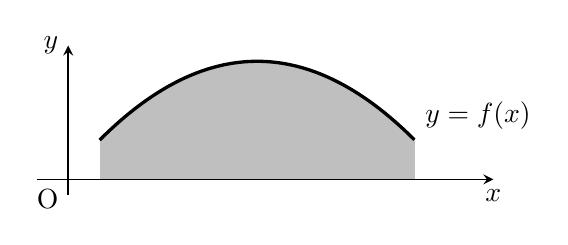
\begin{tikzpicture}[xscale=2]
 \fill[lightgray] (-1,0)--(-1, 0.51)--(1, 0.51)--(1,0)--cycle;
 \filldraw[fill=lightgray, samples=100,domain=-1:1,very thick]
   plot(\x,-1*\x*\x+1.5) node[above right] {$y=f(x)$};%y=f(x)
 \coordinate[label=below left:O] (O) at (-1.2,0); %原点
 \draw[semithick,->,>=stealth] (-1.4, 0)--(1.5, 0) node[below] {$x$}; %x軸
 \draw[semithick,->,>=stealth] (-1.2, -0.2)--(-1.2, 1.7) node[left] {$y$}; %y軸
\end{tikzpicture}
\endpgfgraphicnamed

% 5分割
\beginpgfgraphicnamed{integral_5slice}
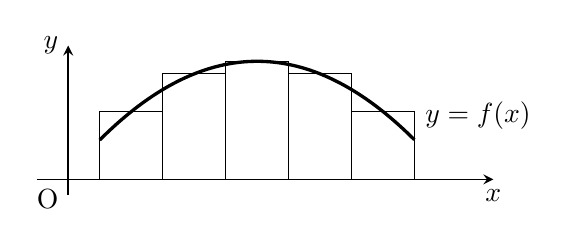
\begin{tikzpicture}[xscale=2]
 \coordinate[label=below left:O] (O) at (-1.2,0); %原点
 \draw[semithick,->,>=stealth] (-1.4, 0)--(1.5, 0) node[below] {$x$}; %x軸
 \draw[semithick,->,>=stealth] (-1.2, -0.2)--(-1.2, 1.7) node[left] {$y$}; %y軸
 
 \draw[samples=100,domain=-1:1,very thick]
   plot(\x,-1*\x*\x+1.5) node[above right] {$y=f(x)$};%y=f(x)
 \foreach [evaluate=\t as \u using \t+0.2]\t in {-1,-0.6,...,0.6}
   \draw (\t,0)--(\t, -1*\u*\u+1.5)--(\t+0.4,-1*\u*\u+1.5)--(\t+0.4,0);
\end{tikzpicture}
\endpgfgraphicnamed

% 10分割
\beginpgfgraphicnamed{integral_10slice}
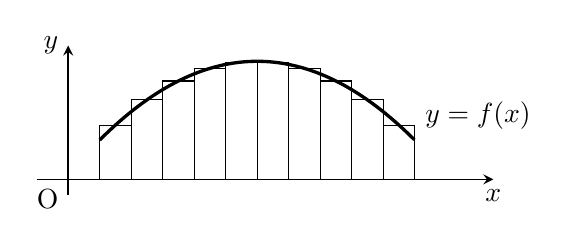
\begin{tikzpicture}[xscale=2]
 \coordinate[label=below left:O] (O) at (-1.2,0); %原点
 \draw[semithick,->,>=stealth] (-1.4, 0)--(1.5, 0) node[below] {$x$}; %x軸
 \draw[semithick,->,>=stealth] (-1.2, -0.2)--(-1.2, 1.7) node[left] {$y$}; %y軸
 
 \draw[samples=100,domain=-1:1,very thick]
   plot(\x,-1*\x*\x+1.5) node[above right] {$y=f(x)$}; %y=f(x)
 \foreach [evaluate=\t as \u using \t+0.1]\t in {-1,-0.8,...,0.8}
   \draw (\t,0)--(\t, -1*\u*\u+1.5)--(\t+0.2,-1*\u*\u+1.5)--(\t+0.2,0);
\end{tikzpicture}
\endpgfgraphicnamed

% 20分割
\beginpgfgraphicnamed{integral_20slice}
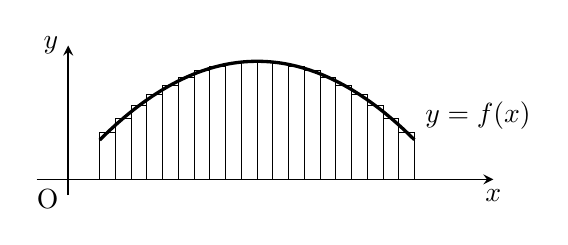
\begin{tikzpicture}[xscale=2]
 \coordinate[label=below left:O] (O) at (-1.2,0); %原点
 \draw[semithick,->,>=stealth] (-1.4, 0)--(1.5, 0) node[below] {$x$}; %x軸
 \draw[semithick,->,>=stealth] (-1.2, -0.2)--(-1.2, 1.7) node[left] {$y$}; %y軸
 
 \draw[samples=100,domain=-1:1,very thick]
   plot(\x,-1*\x*\x+1.5) node[above right] {$y=f(x)$}; %y=f(x)
 \foreach [evaluate=\t as \u using \t+0.05]\t in {-1,-0.9,...,1}
   \draw (\t,0)--(\t, -1*\u*\u+1.5)--(\t+0.1,-1*\u*\u+1.5)--(\t+0.1,0);
\end{tikzpicture}
\endpgfgraphicnamed

\end{document}